\section{Basic Processes}\label{sec:1.2}

Let us begin with a brief qualitative description of the basic processes which come into play in producing a stored electron beam. (See Fig.~\ref{fig:ring})

\begin{figure}[!htb]
	\centering
	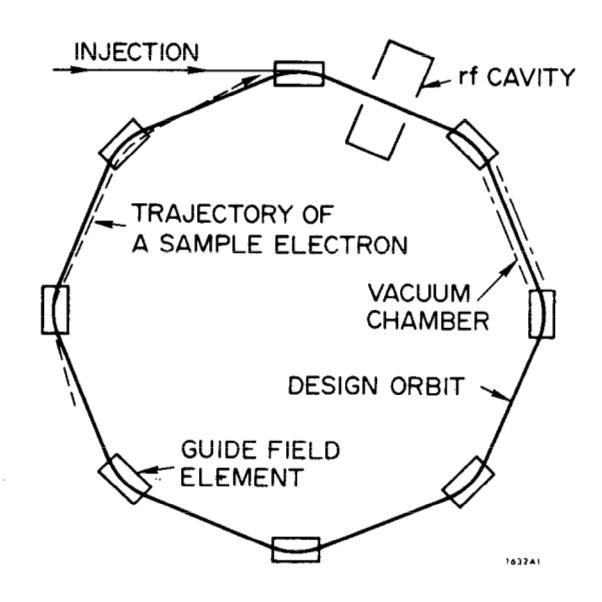
\includegraphics[width=0.6\linewidth]{./Figuras/fig01.jpeg}
	\caption{Schematic diagram of an electron storage ring.}
	\label{fig:ring}
\end{figure}

A short pulse of a beam of electrons is injected into a vacuum chamber embedded in a more-or-less circular \emph{magnetic guide field}. The guide field leads the electrons around in more-or-less closed paths to make a \emph{stored beam}.

The guide field has \emph{focussing} properties which drive all electrons toward an ideal \emph{design orbit} and cause them to execute lateral (radial and vertical) \emph{betatron oscillations} about the ideal closed path.

During each revolution an electron loses a small fraction of its energy by \emph{synchrotron radiation}. For stored electrons this energy loss is compensated for by a corresponding gain of energy from a radio frequency cavity (or from several cavities acting in concert).

The periodic accelerating field collects the electrons into circulating \emph{bunches}, within which the individual electrons oscillate in \emph{longitudinal} position and in energy relative to an ideal reference particle at the center of the bunch. The associated motions in longitudinal position and energy are called the \emph{synchrotron oscillations}.

The energy loss by synchrotron radiation together with the compensating energy gain from the rf cavity gives rise to a slow \emph{radiation damping} of all oscillation amplitudes; the trajectory of each electron tends toward that of an ideal reference particle at the center of the bunch (which moves with constant speed along the design orbit).

Radiation damping does not conserve phase density, so it is possible to inject, successively, many pulses into the neighborhood of the same ideal orbit and obtain high circulating currents from weak sources.

The damping of all oscillation amplitudes is effectively arrested because of a continuous excitation of the oscillations by “noise” in the electron energy, which comes about from the fact that the synchrotron radiation is emitted in photons of discrete energy - the so-called \emph{quantum fluctuations} of the energy loss.

In stationary conditions a balance is reached between quantum excitation and radiation damping, leading to a statistically stationary distribution of the oscillation amplitudes and phases of the electrons in a bunch. The bunch then takes on the aspect of a traveling strip of ribbon which has a stationary “size” and “shape”, with a Gaussian distribution of amplitudes in each of the transverse and longitudinal coordinates (see Fig.~\ref{fig:fig2}). (The shape of a bunch will be different at each azimuthal position because the focussing properties of the guide field vary from place to place, but in the stationary condition the bunch has the same transverse shape at each successive turn for any chosen azimuth).

\begin{figure}[!htb]
	\centering
	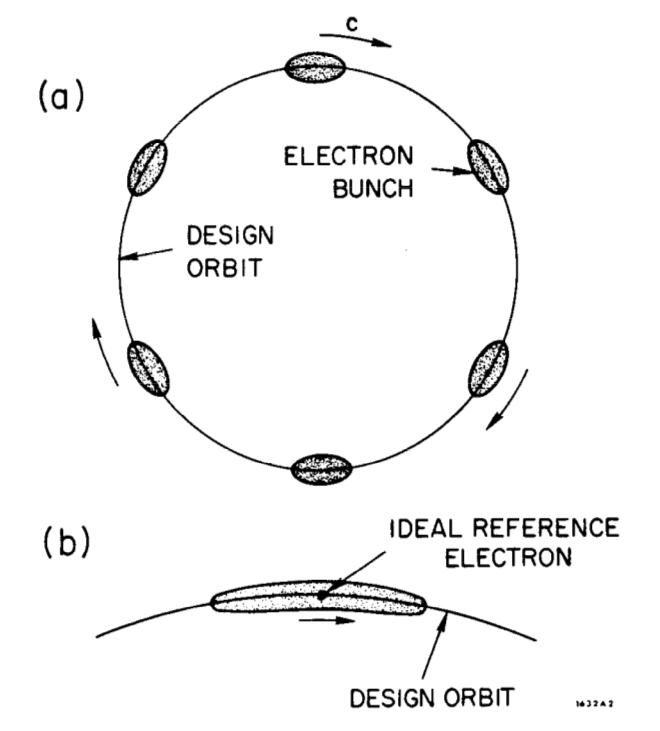
\includegraphics[width=0.55\linewidth]{./Figuras/fig02.jpeg}
	\caption{Circulating bunches in a stored beam.}
	\label{fig:fig2}
\end{figure}

-- For each coordinate of an electron there is some maximum oscillation amplitude above which the electron no longer remains captured in the bunch. We may refer to the range of stable amplitude in each coordinate at its \emph{aperture}. An electron is lost from a bunch when some disturbance increases the amplitude in any coordinate beyond the corresponding aperture limit. The aperture limit for each coordinate may be set by.a physical obstacle which intercepts the electrons, or by nonlinear effects in the focussing forces which lead to unbounded trajectories for large displacements from the ideal reference electron.

-- Electrons may be lost by scattering or energy loss in collisions with molecules of the residual gas in the vacuum chamber, or by a large statistical fluctuation in the quantum excitation of an oscillation amplitude.

The basic processes considered above are the single-particle effects which are primarily responsible for the intrinsic properties of a stored electron beam. Until now I have considered a bunch as a collection of noninteracting electrons each of which moves as though it were alone in the storage ring. Unfortunately,life is not so simple.
